\let\negmedspace\undefined
\let\negthickspace\undefined
\documentclass[journal]{IEEEtran}
\usepackage[a5paper, margin=10mm, onecolumn]{geometry}
%\usepackage{lmodern} % Ensure lmodern is loaded for pdflatex
\usepackage{tfrupee} % Include tfrupee package

\setlength{\headheight}{1cm} % Set the height of the header box
\setlength{\headsep}{0mm}     % Set the distance between the header box and the top of the text

\usepackage{gvv-book}
\usepackage{gvv}
\usepackage{cite}
\usepackage{amsmath,amssymb,amsfonts,amsthm}
\usepackage{algorithmic}
\usepackage{graphicx}
\usepackage{textcomp}
\usepackage{xcolor}
\usepackage{txfonts}
\usepackage{listings}
\usepackage{enumitem}
\usepackage{mathtools}
\usepackage{gensymb}
\usepackage{comment}
\usepackage[breaklinks=true]{hyperref}
\usepackage{tkz-euclide} 
\usepackage{listings}
% \usepackage{gvv}                                        
\def\inputGnumericTable{}                                 
\usepackage[latin1]{inputenc}                                
\usepackage{color}                                            
\usepackage{array}                                            
\usepackage{longtable}                                       
\usepackage{calc}                                             
\usepackage{multirow}                                         
\usepackage{hhline}                                           
\usepackage{ifthen}                                           
\usepackage{lscape}
\begin{document}

\bibliographystyle{IEEEtran}
\vspace{3cm}

\title{9-9.2-29}
\author{EE24BTECH11064 - Harshil Rathan}
% \maketitle
% \newpage
% \bigskip
{\let\newpage\relax\maketitle}

\renewcommand{\thefigure}{\theenumi}
\renewcommand{\thetable}{\theenumi}
\setlength{\intextsep}{10pt} % Space between text and floats


\numberwithin{equation}{enumi}
\numberwithin{figure}{enumi}
\renewcommand{\thetable}{\theenumi}
\textbf{Question}:\\
Using integration, find the area of the region bounded by the line $2y=3x+12$, x-axis and the lines $x=2$ and $x=8$.\\
\solution \\
\begin{table}[h!]
    \centering
    \begin{tabular}[12pt]{ |c| c|}
    \hline
    \textbf{Equations}& \textbf{Given}\\ 
    \hline
     $2y$ & $3x+12$ \\
    \hline 
     $x$ & $2, 8 $\\
    \hline
    \end{tabular}
    \caption{Given Equations}

\end{table}
\begin{align}
     y=\frac{3}{2}x+6
\end{align}
Calculate area between line and $x=2$ and $x=8$\\
\begin{align}    
     \text{Area}=\int_{2}^{8} \left( \frac{3}{2}x + 6 \right) \, dx
     \label{0.2}
\end{align}
\begin{align}
    \int \left( \frac{3}{2}x + 6 \right) \, dx = \frac{3}{2} \cdot \frac{x^2}{2} + 6x = \frac{3}{4}x^2 + 6x
    \label{0.3}
\end{align}
\begin{align}
    \int_{2}^{8} \left( \frac{3}{2}x + 6 \right) \, dx = \left[ \frac{3}{4}x^2 + 6x \right]_{2}^{8}
    \label{0.4}
\end{align}
First, we calculate the upper limit at $x=8$\\
\begin{align}
   \frac{3}{4}(8^2) + 6(8) = \frac{3}{4}(64) + 48 = 48 + 48 = 96 
   \ref{0.4}
\end{align}
Calculate the lower limit at $x=2$\\
\begin{align}
    \frac{3}{4}(2^2) + 6(2) = \frac{3}{4}(4) + 12 = 3 + 12 = 15
    \ref{0.4}
\end{align}
Subtract the lower limit from the upper limit\\
\begin{align}
      \text{Area} = 96 - 15 = 81
      \ref{0.2}
\end{align}
The Area between $2y=3x+12$ and $x=2$, $x=8$ is $81$ units 
\begin{figure}[h!]
   \centering
   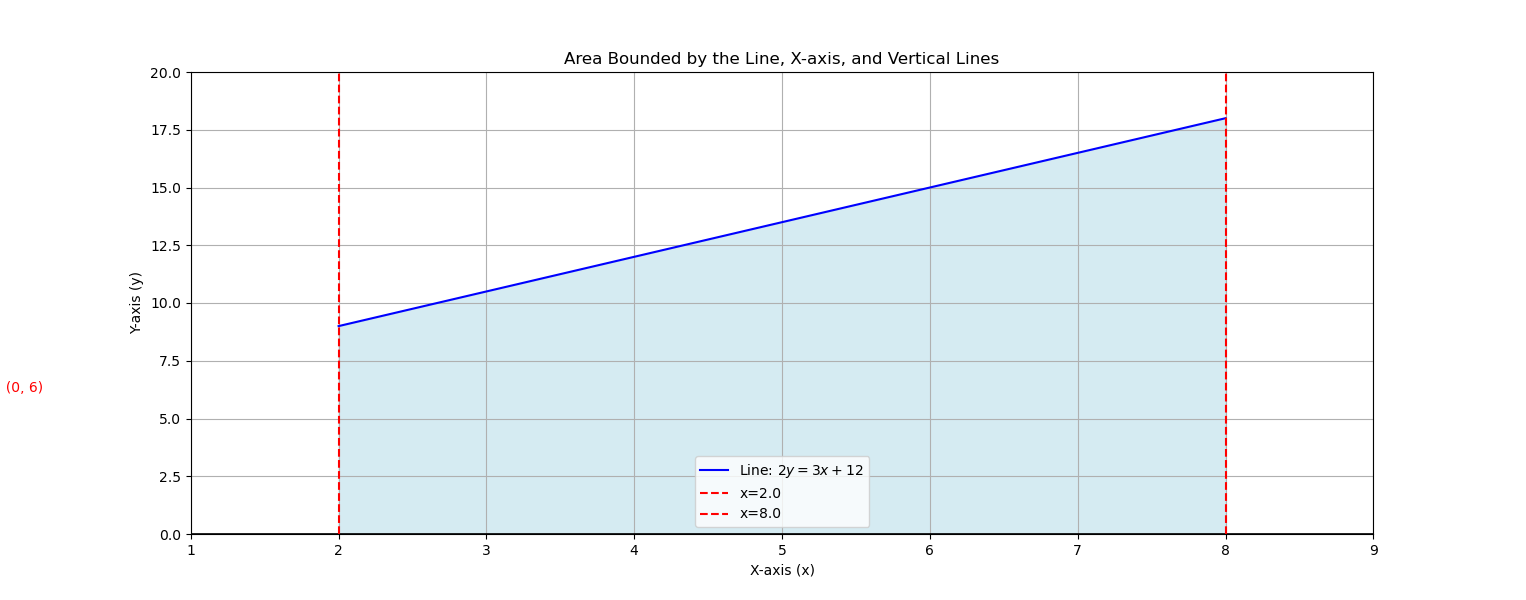
\includegraphics[width=\linewidth]{figs/Figure_1.png}
   \caption{}
   \label{stemplot}
\end{figure}





\end{document}
